\chapter{Mikrokontroladorea}

\vspace{4cm}

Kapitulu honetan, proiektua aurrera eramateko erabili den mikrokontroladorea aztertuko da. Gailu honek dituen barne moduluak ezagutzera emango dira ere, hauen funtzionamendua azalduz eta estazioa behar den bezala funtzionatzeko konfiguratu behar diren erregistroak komentatuz.

\newpage

\section{Atmega328p mikrokontroladorea}

Proiektu honetarako erabili den kontrolagailua, \textbf{Atmega328p}-a izan da. Gailu hau, \textit{Atmel} konpainiak garatutako \textit{megaAVR} serieko potentzia baxuko 8 biteko CMOS mikrokontroladore bat da, AVR-rako hobetutako RISC arkitekturan oinarritutakoa. Mikrokontroladore hau oso ezaguna da, Arduino UNO txartelak erabiltzen baitu.

Arduino UNO plaka oso erabilia da elektronika proiektuen hasiberrian artean, bere merketasuna eta programatzeko erraztasunarengatik. Arduino plataforma handia bihurtu da 2003 urtean Arduino UNO-a atera zutenetik, eta gaur egun hamaika liburutegi eta plaka berri atera dituzte komunitatearen nahiak asetzeko, eta honek erraztasun handiak ematen ditu programatzerako orduan. Izan ere plataformak eskaintzen dituen baliabide hauke guztiak nahiko ilunak dira, programatzerako orduan funtzio sorta bat erabiltzen da eta ez dago argi erabilitako barne moduluen konfigurazioak nolakoak diren. Barne modulu hauen funtzionamendua eta konfigurazioak xehetasun guztiekin aztertu ahal izateko, proiektu honetan Atmega328p-a erregistro mailan programatuko da. 
%*zer da arduino y toda la txapa* *erregistro mailan y todo eso* *Poner las caracteristicas del arduino* y *poner el pinout*.  

\begin{figure}[htb]
	\centering
	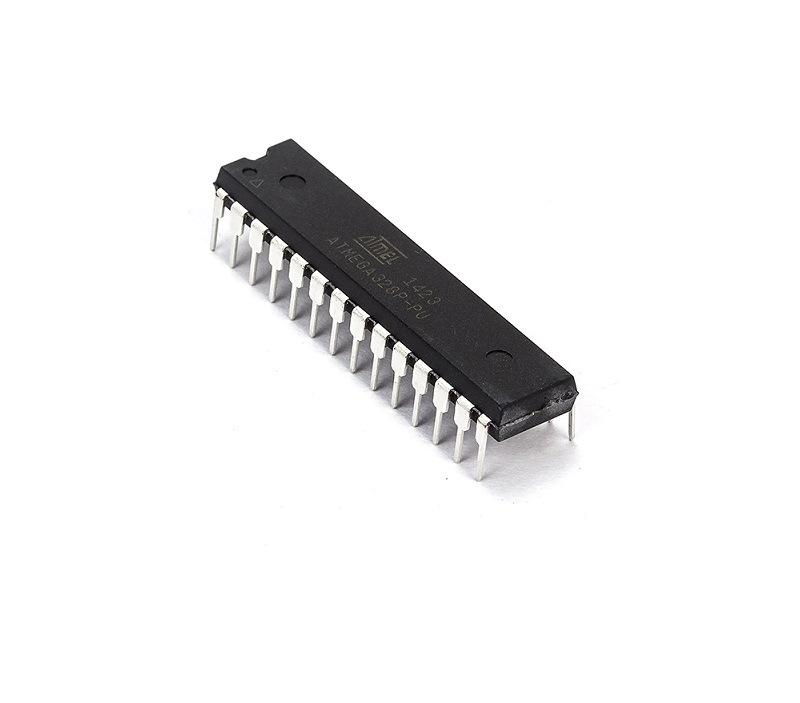
\includegraphics[width=.4\linewidth]{images/atmega.jpeg}
	\caption{\label{fig:bloke_diag} Atmega328p txipa}
\end{figure}

\section{Barne egitura}
Atal honetan, Atmega328p mikrokontroladoreak daukan barne egitura aztertuko dugu. Azpiko \ref{fig:bloke_diag} irudian ikusi daitezke ondoren ikertuko ditugun txiparen osagarri guztiak.

\begin{enumerate}
    \item \textbf{AVR prozesu unitatea:} Hau da mikrokontroladorearen zati garrantzitsuena, programen exekuzio zuzena bermatuko baitu. Prozesu unitateak \textit{Harvard} arkitektura erabiltzen du, programa eta datuentzako bus eta memoria desberdinak erabiliz. Aginduak erloju ziklo bakoitzean exekutatzen dira eta memoriak atzitzeko, kalkuluak egiteko, periferikoak kontrolatzeko eta etenak kudeatzeko gai da.
    \item \textbf{Timerrak:} Guztira 3 timer daude, non horietako bi 8 bitekoak diren eta bestea 16 bitekoa, guztiek prescaler berdina erabiltzen dute, baina konfigurazio desberdinekin. Horretaz gain 6 PWM kanal daude. %PWM kanalak
    \item \textbf{Komunikazio interfazeak:} Hiru desberdin dauzka txip honek, USART, SPI eta TWI. Interfaze hauetako bakoitzak datuak jaso eta bidali ahal izateko aurredefinitutako eta komunikaziorako prest dauden sarrera/irteera pinak erabiltzen dituzte.
    \item \textbf{Memoriak:} Hiru dira Atmega328p-ak dituen memoriak, 32k byteko Programa Flash memoria programak gordetzeko, 2k byteko SRAM memoria bat, programak sortzen dituen aldagaiak gorde ahal izateko eta azkenik 1k byteko EEPROM memoria bat informazio iraungarria gorde ahal izateko.
    \item \textbf{ADC modulua:} seinale analogiko bat, 10 biteko datu batean bihurtzeko gai da (0-tik 1023-ra). Modulu honek 6 sarrera/irteera pin ditu. %analog comparer
\end{enumerate}
\newpage
\begin{figure}[htb]
	\centering
	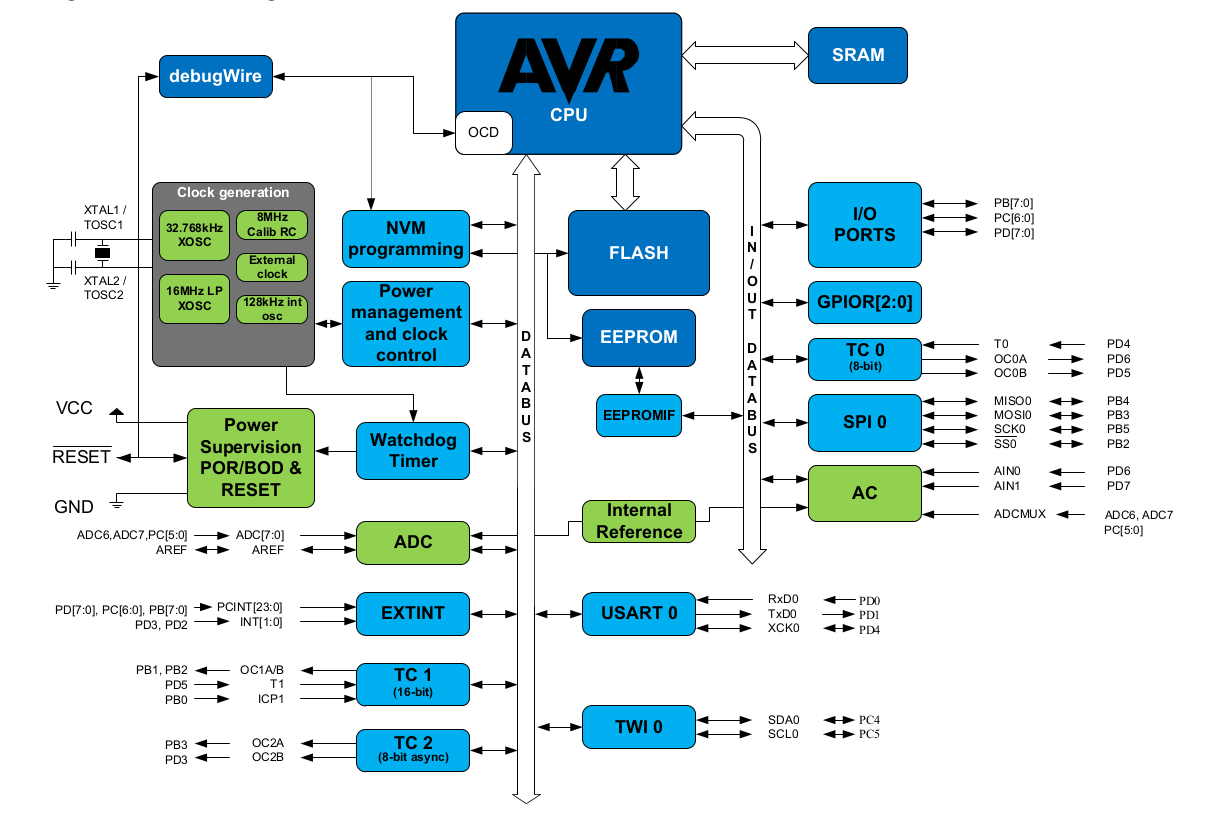
\includegraphics[width=.99\linewidth]{images/bloke_diagrama.png}
	\caption{\label{fig:bloke_diag} Atmega328p txiparen bloke diagrama}
\end{figure}


\section{Sarrera/Irteera hankatxoak}

Atal honetan Atmega328p txipak dituen hankatxoak aztertuko ditugu, guztira 28 dira eta hauetako bakoitza hainbat gauzetarako erabili daitezke. Hona hemen \ref{fig:pinout} irudian agertzen diren hankatxoen azalpena.

\begin{enumerate}
    \item \textbf{VCC: }
    \item \textbf{GND:}
    \item \textbf{PORTB:}
    \item \textbf{PORTC:}
    \item \textbf{PC6/$\overline{RESET}$:}
    \item \textbf{PORTD:}
    \item \textbf{AV$_{CC}$:}
    \item \textbf{AREF:}
    \item \textbf{ADC:}
\end{enumerate}

% azaldu hankatxoak taldeka PCINT, etenak, analog, digitak tx, rx, SDA, SCL, TWI....
\newpage
\begin{figure}[htb]
	\centering
	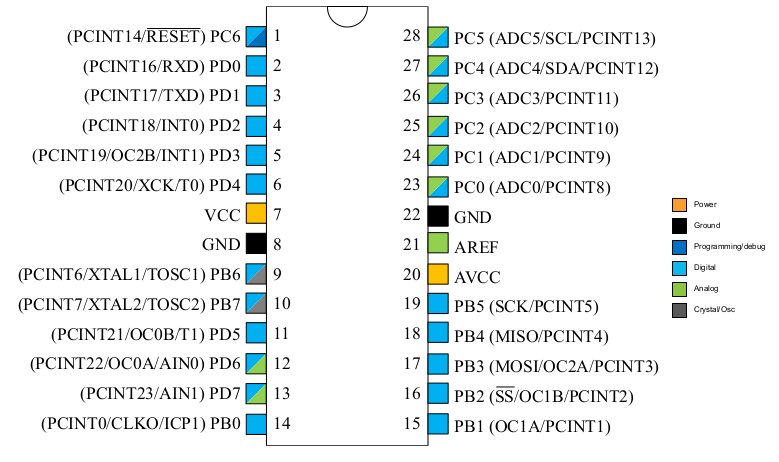
\includegraphics[width=.8\linewidth]{images/pinak.png}
	\caption{\label{fig:pinout} Atmega328p txiparen hankatxoen diagrama}
\end{figure}